\definecolor{cycle1}{HTML}{1f77b4}
\definecolor{cycle2}{HTML}{ff7f0e}
\definecolor{cycle3}{HTML}{2ca02c}
\definecolor{cycle4}{HTML}{d62728}
\definecolor{cycle5}{HTML}{9467bd}
\definecolor{cycle6}{HTML}{8c564b}
\definecolor{cycle7}{HTML}{e377c2}
\definecolor{cycle8}{HTML}{7f7f7f}
\definecolor{cycle9}{HTML}{bcbd22}
\definecolor{cycle10}{HTML}{17becf}


\begin{figure}[t]
\centering
\includegraphics[width=1.0\linewidth]{length_bleu.pdf}
\caption{Effect from different lengths $m$ in FAST. } 
\label{fig:length_bleu}
\end{figure}


\begin{figure}[t]
\centering
\pgfplotsset{width=8.1cm,height=5cm,
    every axis y label/.append style={at={(-0.1,0.5)}},%全局图框
    every axis/.append style={line width=0.6pt},
}
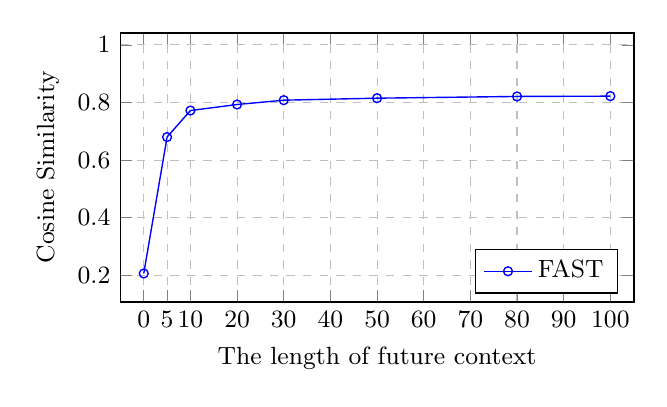
\begin{tikzpicture}[baseline]
\begin{axis}[
    ylabel=Cosine Similarity,%y轴标签名
    xlabel=The length of future context,
    % every axis/.append style={line width=0.4pt},%边框线段粗细
    enlargelimits=0.05,
    legend pos=south east,% 图例的位置
    legend style={font=\small},
    font=\small,
    ymajorgrids=true,%y轴网格线
    xmajorgrids=true,%x轴网格线
    grid style=dashed,%虚线
    ymin=0.15, ymax = 1.0,
    xtick={0,5,10,20,30,40,50,60,70,80,90,100},
    %xmin=500, xmax = 3000,
]
\addplot[color=blue,mark=o, mark size=1.6pt,line width=0.5pt] coordinates{(0,0.206)(5,0.68)(10,0.772)(20,0.793)(30,0.808)(50,0.815)(80,0.821)(100,0.822)};

\legend{FAST,FAI}
\end{axis}
\end{tikzpicture}
\caption{Effect from different lengths $m$ on the $\Bar{s}_{t,t}$ of the last position of streaming speech.}
\label{fig:length_cos}
\end{figure}